\documentclass[10pt,a4paper]{article}

\usepackage[hidelinks]{hyperref}
\usepackage{amsmath}
\usepackage[margin=1.5in]{geometry}
\usepackage{graphicx}
\usepackage{caption}

\begin{document}
\twocolumn
\title{Mobile Robot Systems Mini Project 5}
\author{Sam Sully (sjs252), Paul Durbaba (pd452), Luke Dunsmore (ldd25)}
\date{Lent 2020}
\maketitle
\section{Introduction}
Our project seeks to control a number of robots in a collaborative multi-robot system in order to cover a map in the shortest time. In order to do this the robots will need to localise so that they can report their positions, and thus covered areas. We implement the collaborative localisation strategy presented in Dr Prorok's thesis~\cite{prorok} and compare it with the simpler particle filter implemented in exercise 1 of the Mobile Robots System course.
\section{Localisation}
This section of the project was developed by Sam Sully (sjs252). The approach used was a combination of the sensor-based particle filter used in exercise 1 and the range and bearing approach presented in Dr Prorok's thesis~\cite{prorok}.

The particle filter works by randomly picking samples (particles) from a proposal distribution and then computing the probability that each particle is correct based on measurements from the robot's sensors. We then re-sample the particles, replacing the less likely ones with more likely ones.

Our approach used a known map, the range sensors measurements from the robot's LIDAR and the range and bearing measurements between robots. The weight of the robot is first calculated using the range sensor measurements using a Gaussian measurement model. The weight is given by the below formula:
\[
	w_i = \prod_{s_{j} \in \mathrm{Sensors}}\Phi(R(i,j), s_{ij}, \sigma^2)
\]
where $w_i$ is the weight of particle $i$, $s_{ij}$ is the distance recorded by sensor $j$ on the robot, $\Phi(x,\mu,\sigma)$ is the Gaussian PDF with mean $\mu$ and standard deviation $\sigma$ and $R(i,j)$ is the ray traced distance from particle $i$ in the direction of sensor $j$.

This can effectively be summarised as the product of the Gaussian PDF for each sensor where the mean is the sensor's observed value and the input to the PDF is the raytraced distance from that particle.

We then refine the weight if there are any other robots in range and line-of-sight (these robots are referred to as the neighbours, the set $N_i$ represents robot $i$'s neighbours.). To do this we compute a second weight, $\bar{w_i}$ using the below formula:
\[
	\bar{w_i} = \prod_{r_j \in N_i}\sum_{p_k \in r_j}\Phi\left(
	\begin{bmatrix}
		D_i(p_k)\\
		\Theta_i(p_k)
	\end{bmatrix},
	\begin{bmatrix}
		d_j\\
		\theta_j
	\end{bmatrix},
	\xi
	\right)
\]
where $p_k$ ranges over the set of particles from robot $r_j$, $d_j$ is the received distance between this robot and robot $r_j$, $\theta_j$ is the received bearing of this robot from $r_j$, $D_i(p_k)$ is the distance between the particle $i$ on this robot and the particle $p_k$ from the other robot, $\Theta_i(p_k)$ is the bearing between the particle $i$ and the particle $p_k$ on the other robot and $\xi$ is the covariance matrix. I have omitted normalisation factors.

This can be explained as taking the product of the sums of the bivariate Gaussian PDF for each particle in each robot in range where the means are the range reported from that robot and the bearing reported from that robot and the input to the PDF is the calculated values of range and bearing based on that particle's pose and the local particle's pose.

We then take these two quantities, $w_i$ and $\bar{w_i}$ and multiply them together to get the final weight.

We will now compare the performance of the collaborative localisation and the non-collaborative approach. To do this we created a test environment where two robots were already well-localised and one was not. Figure 1 shows the localisation error over time with the collaborative approach while figure 2 shows the error for the standard (non-collaborative) approach. As can be clearly seen the collaborative approach yields a much faster convergence and a lower error following convergence.
\begin{figure}
	\centering
	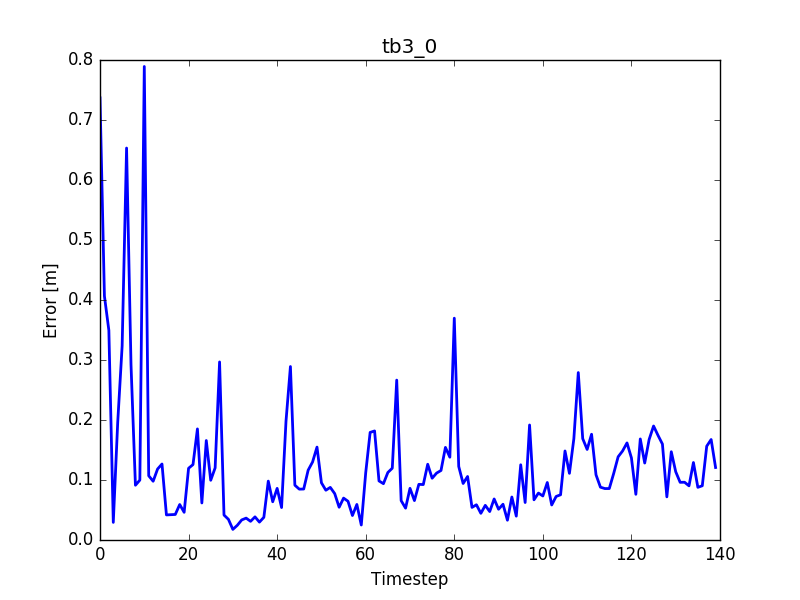
\includegraphics[width=\columnwidth]{figure_l1.png}
	\caption{Error of localisation estimation over time using collaborative approach.}
\end{figure}
\begin{figure}
	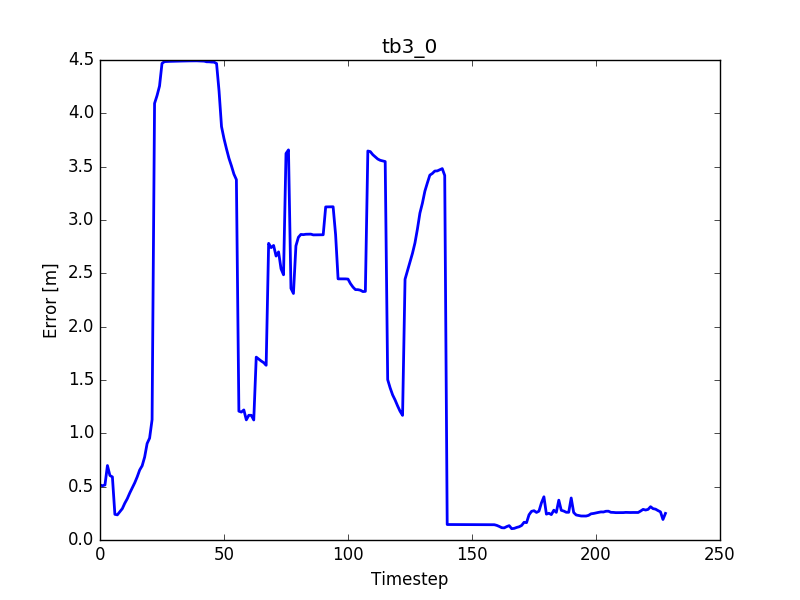
\includegraphics[width=\columnwidth]{figure_l2.png}
	\caption{Error of localisation estimation over time using standard approach.}
\end{figure}
\section{Centralised Navigation}
\section{Decentralised Navigation}
\section{Evaluation}
\section{Conclusions}
\begin{thebibliography}{9}
\bibitem{prorok} A. Prorok, Models and Algorithms for Ultra-Wideband Localization in Single- and Multi-Robot Systems. 2013.
\end{thebibliography}
\end{document}